 \chapter{Predictive Modelling of Frequent Users}
 \label{chpt:predictive-modelling}
  \nomenclature[1]{GRU}{Gated recurrent unit}
 
 
  \newcommand\MyBox[2]{
  \fbox{\lower0.75cm
    \vbox to 1.7cm{\vfil
      \hbox to 1.7cm{\hfil\parbox{1.4cm}{#1\\#2}\hfil}
      \vfil}%
  }%
}
 

\section{Introduction}


















A key objective at this stage of the research is to derive the optimal neural network architecture for the purposes of medical diagnostics within the scope of this thesis. To this end we conducted a series of comparisons between three different types of neural network over a range of parameters and hyperparameters, in relation to the classification of textual notes, and measured the optimal performance of each. The textual notes themselves were presented to each of these classifiers in different data forms in order to ascertain the ideal format for their processing, and whether a marked difference between the different classifiers emerges based upon the format of the data provided to them. 




In order to test our hypothesis that FTN could provide effective features for generating predictive models to determine frequent users, we sought to develop a proof of concept centred upon deep learning methodologies. A number of questions needed to be addressed in relation to the development of an ANN classifier. While ANNs\index{Artificial Neural Networks} have gained considerable attention in recent years, there is no universal design that can be employed, irrespective of domain or data type, that is guaranteed to produce optimal results. Moreover this extends beyond considerations relating to the architecture of the ANN itself, but includes the manner in which data is to be presented to the ANN.  

\hl{The contents of this chapter were in part published in EMBC 2019 `Outlier Detection in Health Record Free-Text Using Deep Learning'} \cite{wallace2019outlier} and `Analysis of EHR Free-text Data with Supervised Deep Neural Networks' \cite{wallace2018analysis} in CSCE 2018 which sought to identify means of successfully classifying frequent user cases using neural networks.

This chapter will describe the measures taken to address these stages of the research: how the data was prepared for classification, how competing ANN architectures performed with FTN data, and how different data implementations affected classifier effectiveness. 

The aim of this section is to provide a key component of a decision support, namely the means to predict patients that are likely to require elevated levels of care. For training purposes, this is defined as any patient who called or was referred to the OOHC\index{Out-of-hours Health Care} in question more than 40 times in a calendar year. \hl{This figure was chosen as a transitory working figure while a more permanent definition of frequent user was obtained in consultation with Caredoc. This figure was adequate in its role in determining a suitable model for case classification.}  

This research used the popular open-source library Tensorflow \index{Tensorflow}1.14.0 \cite{tensorflow2015-whitepaper}, with Python 3.6.6, packaged by conda-forge in the development of the ANN architectures described below. The CUDA API V9 was also used for interfacing with a graphics processing unit for these tests \cite{nvidia2017cuda}. The software these models were built and tested on was compiled with MSC v.1900 64 bit (AMD64).



\section{Architecture Choice}
\label{M}

\subsection{Data Processing}
\label{DP}


In the scope of the investigation conducted by this part of the thesis we excluded all normalised data, such as information relating to the age, or sex of the patient, or information concerning the urgency of or amount of time taken in handling patients' calls. This section exclusively focuses on free-text data, which, notwithstanding  its huge potential in medical analytics, has traditionally been the most difficult source of medical data for use in the context of machine learning. The exclusive aim of this section is to determine the optimal configuration of data and neural network hierarchy for the classification of free-text derived from EHR\index{Electronic Health Record} systems.  

In processing the data we cleaned and tokenised the already anonymised free-text notes (as described in Chapter \ref{chpt:medicial-dataset}).  Cleaning of free-text\index{free-text} included the conversion of unicode to ASCII, the removal of noise (such as the use of symbols to emphasise certain words within the text). We developed our own tokenisation program as our data proved too dissimilar from the data that the majority of off-the-shelf tokenenisers were designed for (e.g. typical Twitter text). Measures that were developed included the disambiguation of words, numbers, and symbols. Where appropriate, symbols and letters which represented words were substituted by their real-world equivalents. As such, a section of text that reads ``temp+++! - 1/2diazepam, tdsx5" would be changed to `` temp ++ 1/2 diazepam , tds * 5". These cleaning and tokenisation processes were designed to be conservative, and were by no means exhaustive in their approach. For instance, within the scope of this section's investigation, no attempt was made to alter the free-text in order to correct spelling errors, disambiguate drug names, or unroll acronyms. Each of the data forms that the free text was converted into (such as word embeddings or list of characters) used this cleaned and tokenised data as its base.

\begin{figure}[htbp]
   \begin{center}

 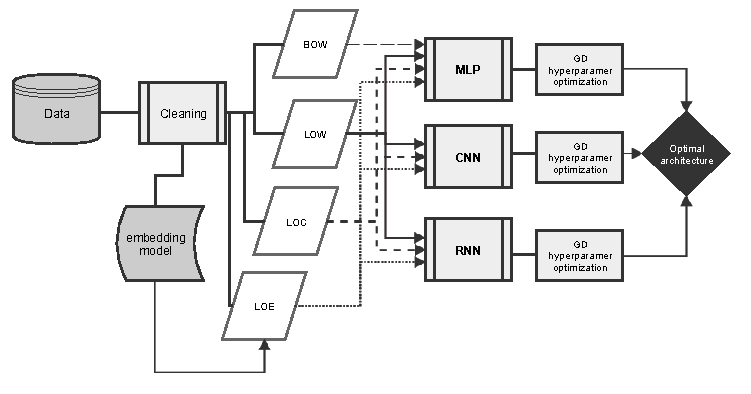
\includegraphics[width=1.0\textwidth]{scheme-lstm1.pdf} 

 \caption{Model for ANN\index{Artificial Neural Networks} testing.}
 \label{fig:ANN-model}
  \end{center}
\end{figure}
 
Data was converted into four mutually exclusive structures: namely bag-of-words (BOW\index{Bag-of-words representation}), list of characters (LOC), list of words (LOW), and list of word embeddings (LOE), as can be seen in Figure \ref{fig:ANN-model}. Each of the data formats has potential merits and demerits in terms of their potential capacity to provide useful representations of patient cases for the purposes of classification. Most of the formats include either implicit or explicit contextual information, with bag-of-words alone being formed of an entirely unstructured representation of patient cases. As mentioned in the related research in Section \ref{section:ANN-(theory)}, bag-of-words is a very popular model for use with this type of task. However, due to its unstructured nature, bag-of-words was only suitable for use in conjunction with the multilayer perceptron ANNs\index{Artificial Neural Networks}. List-of-words and list-of-characters are representations of the data at either a lexeme or character level. Unlike bag-of-words, the structure inherited from the patient cases was maintained. 

FTN attributes (visible in Table \ref{table:free-text}) were appended to one another for each separate case for the generation of input data, as described in Section \ref{section:free-text-description}. Training data was produced using downsampling in order to produce a dataset evenly balanced between positive and negative cases. This approach was necessary in order that domination by a majority class be avoided during training. 

\subsubsection{Length and channels}

To the end of processing FTN\index{free-text} data for use with ANN models this thesis borrows a concept more usually associated with image classification. The term `channel' typically refers to the value (or colour) of an individual pixel being analysed. For the purposes of the FTN data, `channel' refers to the value that the individual token possesses. The actual upshot of this depends on the specific data being considered. In the list-of-characters representation, `channels' relates to the range of ASCII values available. For the BOW\index{Bag-of-words representation} and list-of-words representations, `channels' refers to one-hot encoding of words. Finally, for the word embedding model, `channels' refers to the dimensions of the word embedding. 

It was necessary for reasons of practical consideration to put a fixed upper limit on both the number of channels and the volume of input being examined. For all representations this related to a size of one hundred, for both `channels', and length. In terms of channel number, for both BOW\index{Bag-of-words representation} and list-of-words this correlated to the top one hundred words by frequency in the corpus. For list-of-words, list-of-characters, and list-of-word-embeddings the length of input related to the first one hundred instances of each respective data-type encountered in the associated case FTN. If the input was less than one hundred in length, the input would be padded with zeroes to make up the deficit. If the input was longer than one hundred of its respective data representation, that additional information would be discarded. 

\subsubsection{Word Embeddings}

A significant number of rule-based and statistical language processing algorithms regard
words as atomic symbols. In natural language contexts, such as that found in FTN, this translates to a very sparse representation of the vocabulary. This `one-hot' encoding of lexical information does not document the similarity between any of these symbols. For instance, `chesty' and `wheezing' would from this point of view have no relationship with one another. The practical implication of this is that symbols which appear infrequently are liable to have little impact on algorithmic performance, even if they represent strong information gain. For one thing, even if the particular feature selection technique that is used manages to preserve these data when presenting material to the ML application, their very infrequency would make it less likely for the ML application to have sufficient examples from which to learn these symbols' importance. Moreover, such representations fail to provide information relating to   distributional semantics or co-occurrence statistics. Co-occurrence can be somewhat addressed using N-gram representations. Although N-grams (for instance 2-gram representations) are not considered as part of the testing process in this section, this role is, to all intents and purposes, performed by the LOW representation of the FTN, which essentially preserves co-occurrence information.    

Unsupervised learning using neural networks to create vector based word embeddings has become a very popular means of addressing this particular issue. To this end Word2Vec was used, trained in the manner described in Section \ref{section:word_embeddings}.

%While this approach was necessary, insofar that domination by a majority class had to be avoided during training, this produced a significant prospect for overfitting\index{Overfitting}. 




%How many channels?

\subsection{Hyperparameter optimisation}
\label{section-hyperparemter-optimisation}


  





Choice of hyperparameters can be crucial to the effectiveness of a particular ANN architecture. This becomes a limiting factor due to the fact that suitable hyperparameters may not be known \textit{a priori} \cite{zhou2018exploring,zheng2019hyperparameter}. Unfortunately, choice of hyperparameters is subject to high dimensionality.  Furthermore, tuning of a single hyperparameter may affect the performance of another hyperparameter; therefore tuning in isolation may not necessarily be effective. 

% Please add the following required packages to your document preamble:
% \usepackage{booktabs}






The most simple approach to finding the correct combination of hyperparameters is to perform an exhaustive search across all combinations of hyperparameters. This methodology, known as Grid Search \cite{goodfellow2016deep}, is only suitable within a narrow subset of hyperparamers. Instead, Bayesian optimisation for hyperparameters was performed \cite{snoek2012practical}. Expected improvement can be defined as


\begin{equation}
EIy\textsuperscript{*}(x) = \int_{-\infty}^{y\textsuperscript{*}}(y\textsuperscript{*} -  y)p(y|x)dy
\end{equation}

Where \textit{y}\textsuperscript{*} is a threshold value for the objective function, \textit{y} is the actual value of the objective function, and \textit{p}(\textit{y}|\textit{x}) is the surrogate model.



This model was used to obtain the hyperparameters of hidden layers in relation to the number of layers, number of hidden units, learning rate, activation function, and optimisation function used within each of the three types of ANN. The search space (which is detailed in Table \ref{table:hyperparameter-tuning}) for both RNN\index{Recurrent Neural Network} and CNN\index{Convolutional Neural Networks} featured dropout, while CNN\index{Convolutional Neural Networks} optimisation also included filter, kernel and pool sizes. 

\begin{table}[htbp]

\caption{Search space for hyperparameters.}
\begin{center}
\begin{tabular}{@{}clc@{}}
\cmidrule(r){1-1} \cmidrule(l){3-3}
\textbf{Activation function} & \textbf{} & \textbf{Optimiser} \\ \cmidrule(r){1-1} \cmidrule(l){3-3} 
sigmoid                      &           & Adadelta           \\
hard sigmoid                 &           & Adagrad            \\
relu                         &           & Adam               \\
tanh                         &           & Ftrl               \\
leaky relu                   &           & Gradient Descent   \\ \cmidrule(r){1-1}
                             &           & Momentum           \\ \cmidrule(l){3-3} 
\end{tabular}
\end{center}
\label{table:hyperparameter-tuning}
 \end{table} 

\begin{table}[htbp]
\begin{center}
\begin{tabular}{@{}llc@{}}
\toprule
\textbf{hidden layers}  & \textbf{learning rate}        & \multicolumn{1}{r}{\textbf{dropout}} \\ \midrule
\multicolumn{1}{c}{1-5} & \multicolumn{1}{c}{0.001-1.0} & 0.0-1.0                              \\ \bottomrule
\end{tabular}
\end{center}

\end{table}


\subsection{Long Short-Term Memory}
\label{LSTM}

Long Short-Term Memory (LSTM\index{Long Short-Term Memory}) \cite{gers1999learning}, originally developed to help solve the vanishing gradient problem common in simple RNN\index{Recurrent Neural Network}, is a block that has the capacity to store representations of recent input events. RNN\index{Recurrent Neural Network} have proven application in NLP\index{Natural Language Processing} problems due to capacity of the ANN to remember term dependencies, and could be useful in the interpretation of contextual information in patient cases. As gated units have been proven to be superior to vanilla RNN\index{Recurrent Neural Network}, regardless of context, there was little reason to reestablish this here. A standard LSTM\index{Long Short-Term Memory} unit was implemented, featuring an input gate, an output gate and a forget gate, but the number of LSTM\index{Long Short-Term Memory} units was variable, with the depth to be determined during hyperparameter optimisation.   



\subsection{Selection Outcome}
\label{section-hyperparameter-results}

The output of the classifiers was a binary truth value based on the determined likelihood that the patient case being tested belonged to someone who either currently, or in the near future, would have escalating levels of required care. %A natural issue to arise when 

One hundred different models, based upon different sets of hyperparameters were trained, and ran up to a thousand epochs for each ANN configuration. This experiment was conducted using 45\% of positive cases for training data, 40\% of positive cases for validation data, and 15\% of positive cases for testing data. Training and validation datasets were balanced, while testing used a quarter of the corpus. A total of 3260 cases (or rows) were allocated for training, 2900 cases for validation, and 73584 cases for testing. Testing was conducted using the best configuration, as derived during hyperparameter optimisation.




% Please add the following required packages to your document preamble:
% \usepackage{booktabs}
\begin{table}[htbp]
\centering
\caption{Accuracy results on validation data.}
\begin{tabular}{@{}l|ccc@{}}
\toprule
\textbf{Data}           & \textbf{MLP\index{Multi-Layer Perceptrons}} & \textbf{CNN} & \textbf{RNN\index{Recurrent Neural Network}} \\ \midrule
Bag of Words            & 0.8 $^{\mathrm{a}}$         &            &           \\
List of characters      & 0.64         & 0.72         & 0.73         \\
List of words           & 0.72         & 0.75         & 0.76         \\
List of word embeddings & 0.73         & 0.73         & 0.82         \\ \bottomrule
\multicolumn{4}{c}{}{$^{\mathrm{a}}$Bag of words was used only with MLP}
\end{tabular}
\label{table:hyperparameter-testing}
\end{table}

As shown in Table \ref{table:hyperparameter-testing} above, Multilayer Perceptrons were inferior to both CNN\index{Convolutional Neural Networks} and RNN in relation to contextual information. However, MLP\index{Multi-Layer Perceptrons} performed well using Bag-of-words, underpinning the validity of the frequent usage of this combination, as discussed in Section \ref{section:ANN-(theory)} It was also remarkably fast to train an MLP\index{Multi-Layer Perceptrons} on a simple bag-of-words model, relative to the other models under consideration. 

Character level encoding proved an inferior representation regardless of ANN type. The high dimensionality of feature space was not offset by quality of the data presented to the classifiers, thus generating both long training times and inferior accuracy.

One-hot encoding of lexemes with contextual conservation generated adequate results, and in testing proved the most suitable representation for Convolutional Neural Networks. Although the CNN\index{Convolutional Neural Networks} model achieved good results in all categories, it was nonetheless consistently outperformed by Recurrent Neural Networks using LSTM\index{Long Short-Term Memory}.

\begin{table}[htbp]
\caption{Optimal configuration.}
\begin{center}
\begin{tabular}{|c|c|c|c|c|c|}
\hline


\cline{2-4} 
\textbf{Model} & \textbf{\textit{$\mu$}} & units & layers & $\varphi$ & opt \\
\hline
MLP &  \  0.73639 &  48 &  2 &  leaky relu & GradientDescent  \\
\hline
CNN & 0.002257 & 76 & 3 & relu & Adam   \\
\hline
RNN &0.003186  & 100 & 3 & tanh & GradientDescent   \\ 
\hline
 

\end{tabular}
\label{tab3}
\end{center}
\end{table}




Recurrent Neural Networks using LSTM\index{Long Short-Term Memory} performed well using all data representations. However, the use of word embeddings saw a significant increase in the potential output of this classifier. While significantly more expensive to train than an MLP\index{Multi-Layer Perceptrons} network, this combination was the most successful in classifying patients.


\noindent
\renewcommand\arraystretch{1.5}
\setlength\tabcolsep{0pt}
\begin{table}[htbp]
\caption{Testing results.}
\begin{tabular}{c >{\bfseries}r @{\hspace{0.7em}}c @{\hspace{0.2em}}c @{\hspace{0.7em}}l}
  \multirow{10}{*}{\parbox{1.1cm}{\bfseries\raggedleft actual\\ value}} & 
    & \multicolumn{2}{c}{\bfseries Prediction outcome} & \\
  & & \bfseries p & \bfseries n & \bfseries total 13287 \\
  & p$'$ & \MyBox{443}{} & \MyBox{12844}{} & P$'$ \\[2.2em]
  & n$'$ & \MyBox{108}{} & \MyBox{60189}{} & N$'$ \\
  & total 60297 & P & N &
\end{tabular}
\label{table:LSTM-first-results}
\end{table}

The optimal hyperparameters, listed above in Table \ref{tab3} relate to the Bag-of-Words\index{Bag-of-words representation} model for MLP\index{Multi-Layer Perceptrons}, the List-of-Words model for CNN\index{Convolutional Neural Networks}, and list of word embeddings for LSTM\index{Long Short-Term Memory}. The optimal hyperparameters for CNN\index{Convolutional Neural Networks} included a pool size of 3 and 18 dense units. As the Recurrent Neural Network, with word embeddings, performed best, its results in testing are shown above in the confusion matrix in Table \ref{table:LSTM-first-results}, while the training cost using this configuration is shown in below in Figure \ref{fig1}. A dropout rate of 0.136 was also applied to this network in order to reduce the occurrence of overfitting\index{Overfitting}. Although the results, as described in Table \ref{table:LSTM-first-results}, were at this stage quite modest, the architectural framework for future neural network development within the project had been established.

%Our deep LSTM network achieved precision of 0.82.


\begin{figure}[htbp]
\centerline{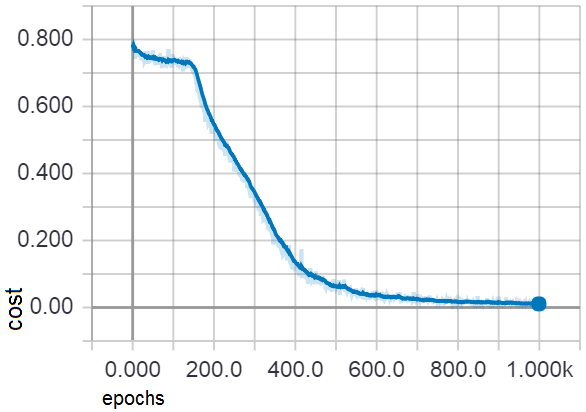
\includegraphics[width=3.0in]{training2.png}}
\caption{Training cost for RNN.}
\label{fig1}
\end{figure}


\subsection{Discussion}


This section above detailed not only that ANNs\index{Artificial Neural Networks} can achieve high quality results in classifying patients from medical free-text, but that not all data representations performed as well as one another. A single data representation was likely to produce different results, depending on the type of ANN it was provided to. Moreover, the performance of any given ANN was largely tied to the specific hyperparameters in use. Applying Bayesian optimisation allowed the application of suitable hyperparameters for use with each of the ANNs\index{Artificial Neural Networks}, and as such determine the most suitable ANN for use with the data under consideration. Of course, merely reporting the hyperparameters which gave the optimal performance does not provide the full story. There were numerous combinations of hyperparameters which prevented any successful training of the respective model. Equally there were numerous combinations which performed well, but had marginally weaker results than the set of hyperparamters reported above. As an aside, it is interesting and somewhat surprising how well MLP\index{Multi-Layer Perceptrons} managed to perform with a character level representation of the dataset (bear in mind that with the balanced class representation of the validation data, that 50\% accuracy is no better than random).

While an n-gram representation of characters would be likely to perform better than the individual character representation, character level representations had clearly been the least effective method of representing case data, regardless of the model employed. This data representation was also an order of magnitude more expensive to train compared to other representations.     

Notwithstanding the mixed quality of data, and even in the absence of individual patient histories, the ANN architectures performed well. This was particularly relevant to the research question of this thesis, which concerns the classification of a cohort for whom there is not a well defined set of symptoms. As such, there was no need to attempt to extract potentially useful features for a machine learning algorithm, but rather allow the neural networks to decide which features were deemed most representative.  

Whilst the classifier performed well in determining frequent-user from non frequent-user cases, the issue remained that the so-called black box model of neural networks creates challenges in interpretability \cite{liu2018improving}. The capacity of a classifier to not merely provide the service of identifying members of a cohort, but to inform medical professions the phenotypes likely to represent certain patients is of specific importance within the domain of medical treatment \cite{london2019artificial,preece2018asking}. Therefore a means to potentially identify the salient features of the FTN that contributed to positive and negative predictions became an objective of our research.



As Recurrent Neural Networks with LSTM\index{Long Short-Term Memory} had outperformed the other ANN architectures listed above, many concerns relating to the hand curation of features were allayed. As a sequential architecture, Recurrent Neural Networks have an inherent appreciation of context \cite{yin2017comparative}. Consequently there was no need to process individual lexemes to represent their specific context. For instance, contextual negation did not have to be processed through the NegEx algorithm \cite{chapman2001simple}, as the RNN\index{Recurrent Neural Network} itself could learn the significance of negation. Unlike rare lexemes (like misspelled medication names), these types of contexts were in plentiful supply. This contextual understanding, supplemented with the semantic information contained within the word embedding representation of the corpus, combined to give a comprehensive approach to the NLP\index{Natural Language Processing} context of the FTN.

Nevertheless, numerous questions remained unanswered. Could superior results be achieved by using an alternative gating technique to LSTM\index{Long Short-Term Memory}; by using a different method of word embedding to Word2Vec\index{Word2Vec} trained on the corpus; or by applying the parameterised data of the corpus as input features to the network? Furthermore this section did not test the corpus using the preprocessing techniques described in Chapter \ref{chpt-preprocessing}. The following sections will address these outstanding issues, including whether increasing the input itself (in terms of either length or dimensionality) might improve results.  



\section{Recurrent Neural Network Application}
\label{RNNA}

\subsection{Data selection}
\label{testing-methodologies}

After consultation with the OOHC\index{Out-of-hours Health Care} in question, the two criteria chosen for classifying frequent users were patients who contact the OOHC\index{Out-of-hours Health Care} more than 50 times in a year (approximately once a week), which will be described as high frequent users, and those that contact the OOHC\index{Out-of-hours Health Care} more than 24 times in a year, which are simply described as frequent users. For the sake of brevity, in the following tables, `threshold' will be abbreviated to \textit{t}. As described in Section \ref{section:frequent-users-rr}, this demarcation between different grades of frequent use is fairly typical in the medical domain. Training, test, and validation sets were split by user and contained 50\%, 25\%, and 25\% of positive cases respectively, where training and validation sets were balanced, and testing set imbalanced. Consequently, when conducting experiments considering frequent users, t(24), training used a total of 7,365 cases, validation used 3,682 cases, and testing used 283,289 cases in total. For experiments considering high frequent users t(50), training used a total of 2,922 cases, validation 1,461, and testing 289,953 cases in total. All results discussed from Section \ref{word-embedding-comparrison} to Section \ref{extending-threshold} were obtained using 5-fold cross validated testing sets \cite{arlot2010survey}.    

\subsection{Word embedding comparison}
\label{word-embedding-comparrison}

\begin{figure}[ht]
   \centering
   \begin{tabular}{@{}c@{\hspace{.5cm}}c@{}}
 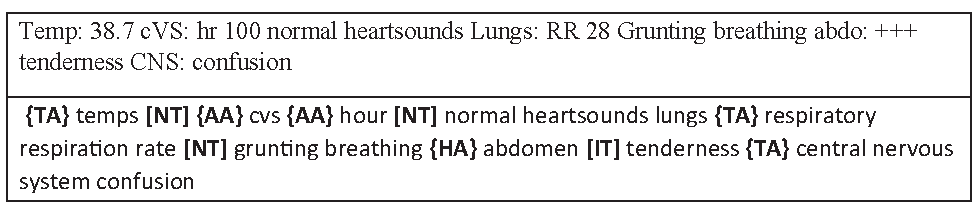
\includegraphics[page=1,width=1.0\textwidth]{embc0.pdf} & 
   \end{tabular}
 \caption{Case with transformation performed, featuring identification and unrolling of contractions,  and identification and replacement of shorthand. }
 \label{fig:text-transormation-1}
\end{figure}

\begin{figure}[ht]
   \centering
   \begin{tabular}{@{}c@{\hspace{.5cm}}c@{}}
 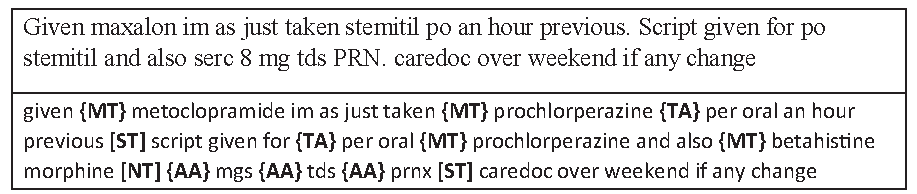
\includegraphics[page=1,width=1.0\textwidth]{embc1-1.pdf} & 
   \end{tabular}
  \caption{Another case with transformations, showing the identification and replacement of medications with generic varieties. }
 \label{fig:text-transormation-2}
\end{figure}  


Although RNN (more specifically using LSTM) had been determined, through the results of Section \ref{section-hyperparameter-results}, to be the most promising model to classify frequent user cases, some questions concerning the data itself remained. Consequently testing was conducted to verify the efficacy of the preprocessing described in Chapter \ref{chpt-preprocessing}. 

The preprocessing techniques described in Chapter \ref{chpt-preprocessing} were applied to the FTN. Two examples of the final representation of text based upon these processing techniques can be seen in Figure \ref{fig:text-transormation-1} and  \ref{fig:text-transormation-2}. In this unrolling of acronyms and abbreviations, and identification and replacement of textual shorthand e.g. `+++', the specific method used to identify and/or transform contractions are added as a feature in of itself.


The word embedding comparison was to be made in relation to the GloVe\index{GloVe} (or Global Vectors) model, which is trained on the non-zero entries of a global word-word co-occurrence matrix, which tabulates how frequently words co-occur with one another \cite{pennington2014glove}.  The Word2Vec\index{Word2Vec} model, described in Section \ref{section:word_embeddings}, was retrained on this version of the text. Again, the GloVe\index{GloVe} model was also trained on both the unpreprocessed and preprocessed form of the corpus. Finally we compared Word2Vec pre-trained on the Google News corpus (3 billion running words) word vector model (3 million 300-dimension English word vectors).
For each of these embeddings a comparison was made of performance on the corpus both before and after the textual transformations described in Tables \ref{table:embedding-comp-24} and \ref{table:embedding-comp-50}.








It was no great surprise that the word embeddings trained on the Google News corpus had inferior performance to those trained on our corpus, as the register used in clinical notes deviates significantly from standard linguistic formulation. While textual transformations performed concerning the unrolling of acronyms would have improved the accuracy of this model, other textual transformations (like medication reconciliation) wouldn't have had any noticeable impact, while others (like contraction clustering) would likely have had a negative impact on this particular model's performance. 

\begin{table}[ht]

\setlength{\tabcolsep}{9pt}
      \centering
\caption{Performance relating to word embedding method\index{GloVe}: t(24).}
\label{table:embedding-comp-24}
      \resizebox{\columnwidth}{!}{%
\begin{tabular}{@{}lcccccc@{}}
\toprule
                     & \multicolumn{2}{c}{\textbf{Unpreprocessed}} & \multicolumn{2}{c}{\textbf{Preprocessed }} \\ \midrule
            & PPV                  & NPV                  & PPV                 & NPV                 \\
\textit{W2V}          & 0.66$\pm 0.018$ &    0.72$\pm 0.044$&  0.76$\pm 0.034$     & 0.74$\pm 0.04$                    \\
\textit{GloVe}       & 0.64$\pm 0.077$  &   0.75$\pm 0.073$&  0.72$\pm 0.022$     & 0.76$\pm 0.03$                   \\
\textit{Google News} & 0.62$\pm 0.037$  &   0.69$\pm 0.051$&  0.69$\pm 0.043$      & 0.74$\pm 0.05$                    \\ \bottomrule
\end{tabular}
}
\end{table}

\begin{table}[ht]

\setlength{\tabcolsep}{9pt}
      \centering
\caption{Performance relating to word embedding method\index{GloVe}: t(50).}
\label{table:embedding-comp-50}
      \resizebox{\columnwidth}{!}{%
\begin{tabular}{@{}lcccccc@{}}
\toprule
                     & \multicolumn{2}{c}{\textbf{Unpreprocessed}} & \multicolumn{2}{c}{\textbf{Preprocessed }} \\ \midrule
            & PPV                  & NPV                  & PPV                 & NPV                 \\
\textit{W2V}         & 0.81$\pm 0.013$     & 0.82$\pm 0.01$ & 0.85$\pm 0.016$     & 0.85$\pm 0.028$                   \\
\textit{Glove}     & 0.82$\pm 0.022$     & 0.81$\pm 0.019$ & 0.84$\pm 0.026$     & 0.81$\pm 0.022$                  \\
\textit{Google News} & 0.76$\pm 0.026$     & 0.79$\pm 0.009$ & 0.75$\pm 0.037$     & 0.80$\pm 0.016$                   \\ \bottomrule
\end{tabular}
}
\end{table}

Textual transformation of the clinical notes, as seen in Figures \ref{fig:text-transormation-1} and \ref{fig:text-transormation-2}, had a clear positive impact on both  the precision and negative predictive performance of the different models (with the exception of the pretrained model's precision in relation to high frequent users). Note that these transformations are designed primarily to improve classification accuracy, irrespective of human intelligibility. The divergence in performance between the three types of word embeddings used was interesting, but ultimately indicated that Word2Vec\index{Word2Vec} trained on the corpus was the most reliable of those tested.






\subsection{Gating comparison}

Gated Recurrent Units (GRU\index{Gated Recurrent Units}) are a more recent method of implementing gating, relative to LSTM\index{Long Short-Term Memory}, but feature fewer parameters \cite{cho2014learning}. As both architectures looked promising for use in relation to unstructured text \cite{bansal2016ask}, our tests featured a comparison of the performance of these respective  









\newmdenv[bottomline=false]{topbot}
\newmdenv[topline=false]{bottombot}

\begin{landscape}
   \begin{figure*}[tpb]
   
      \centering
      \begin{topbot}

      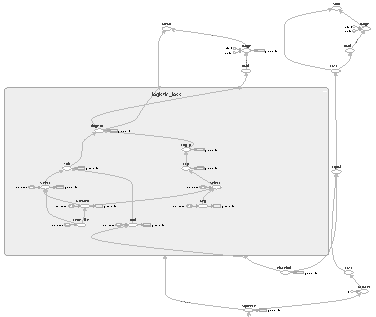
\includegraphics[page=1,width=0.75\textwidth]{scheme-tensorboard-0(1)(half-0).pdf}
      \end{topbot}
      

   \end{figure*}
\end{landscape}   

\begin{landscape}
   \begin{figure*}[tpb]
   
      \centering
      \begin{bottombot}

      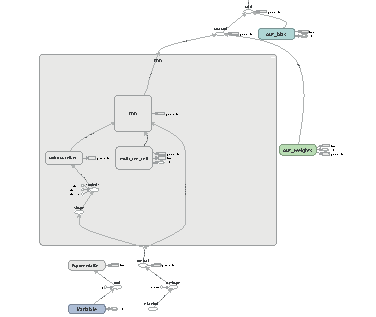
\includegraphics[page=1,width=0.75\textwidth]{scheme-tensorboard-0(1)(half-1).pdf}
      \end{bottombot}
      \caption{Schematic representation of neural network architecture.}
      \label{fig:scheme-tensorboard}
   \end{figure*}
\end{landscape}   

\noindent models. The output of the ANNs\index{Artificial Neural Networks} was a continuous value reflecting the determined likelihood that the case belonged to a frequent user.

\subsubsection{Channel and word length}

Varying the size of channel or input length had not yet been considered as part of ANN testing. While this was an area that merited investigation in its own right, the matter was given particular attention given the effect of preprocessing. Notwithstanding the fact that most significant findings are likely to be written by nurses or doctors at the top of FTN notes, \hl{as elaborated in Section} \ref{section:preproccesing-impact-on-corpus}, the average size of text within FTN\index{free-text} had increased significantly. This heightened the perceived possibility of potentially valuable information being excluded from consideration due to the fixed length of input. Somewhat similarly, testing had not yet excluded the possibility of increased predictive performance by raising the ceiling of dimensionality of word embedding input.  


A further question related to the potential impact that including the parameterised data, described in Section \ref{section:dataset-description}, might have upon the model. The actual means of providing this data to the classifier was predominantly limited to appending this data to the input stream. However, it was hypothesised that providing the model with case data relating to: the age of the patient that the case was related to, the medical card status of the patient, the sex of the patient, the priority ascribed to the case, the time of day that the case had taken place, and the amount of time that the case had lasted might make a significant improvement to the classification accuracy. In counterpoint, the impact of simply adding random values in lieu of these parameterised data was assessed as part of testing. Both parameterised data and noise was prepended to the input stream. 



These series of experiments seemed an ideal venue in which to compare the performance of the LSTM\index{Long Short-Term Memory} and GRU\index{Gated Recurrent Units} gating techniques, and consequently all sets of variables described above were tested against both the LSTM\index{Long Short-Term Memory} and GRU\index{Gated Recurrent Units} models. Both the GRU\index{Gated Recurrent Units} and LSTM\index{Long Short-Term Memory} models were subject to hyperparameter optimisation prior to these experiments (though hyperparamters had already been derived for the LSTM\index{Long Short-Term Memory} model, changes in both the data, and the RNN\index{Recurrent Neural Network} cells that the model was composed of, warranted a fresh round of hyperparameter testing).       


%While dropout was considered as part of the search space of hyperparameters that were subject to Bayesian hyperparameter optimisation (along with the number of layers, learning rate, activation function, and optimisation function used within the ANN), we also sought another potential means to counter overfitting\index{Overfitting}. Our approach was to deliberately prepend the vector data input with noise, to see if this would improve ultimate testing results. This was tested against the addition of normalised features derived from the corpus. Although these normalised features were quite limited in scope, it was hypothesised that the introduction of these features, such as patient age and gender, might improve classification performance. 







%\begin{figure}[htbp]
% \caption{Graph of Recurrent Neural Network featuring LSTM}
%   \begin{center}
%
% 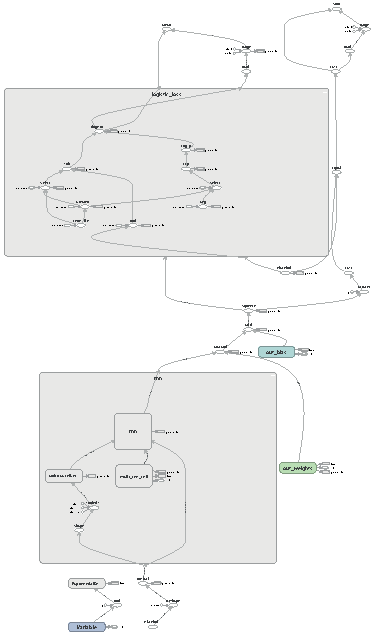
\includegraphics[width=1.14\textwidth]{Figs/scheme-tensorboard-0(1).pdf} 
%
%
% \label{fig:scheme-tensorboard}
%  \end{center}
%\end{figure}







\subsection{Methodology}



Both RNN\index{Recurrent Neural Network} models had batch sizes of 100, while weights were set using He / MRSA initialisation \cite{he2004initialization}. This is different from Section \ref{section-hyperparemter-optimisation} where weights were simply set by a pseudo random number generation. Hyperparameters were again derived using Bayesian optimisation (as described in Section \ref{section-hyperparemter-optimisation}) 


The structure and set of hyperparameters determined through Bayesian optimisation to be the most successful, and used pursuant to the ultimate classification of patients in relation to this chapter, was a Recurrent Neural Network featuring a four layer LSTM\index{Long Short-Term Memory} with a learning rate of 0.001, dropout of 0.3, batch size of 100, and using the Adam optimiser \cite{kingma2014adam}. The alternative Recurrent Neural Network tested featured five layer GRU\index{Gated Recurrent Units}, with learning rate of 0.009, dropout of 0.25, and using the Adagrad optimiser \cite{duchi2011adaptive}. It was uncertain whether increasing the length of input (maximum number of lexemes considered in each case) and channels (the dimensionality of word embeddings) would improve results, and as such, these were also tested. Holdout data related exclusively to cases of patients not featured in training.


\begin{table}[ht]
\caption{Testing hyperparameters.}
\setlength{\tabcolsep}{9pt}
\centering
\resizebox{\textwidth}{!}{%
\begin{tabular}{@{}lcc@{}}
\toprule
                    & \textbf{Long-Short Term Memory} & \textbf{Gated Recurrent Units} \\ \midrule
Learning Rate       & 0.001                           & 0.009                         \\
Number of Layers    & 4                               & 5                             \\
Activation function & relu                            & relu                          \\
Optimiser           & Adam                            & Adagrad                       \\
Dropout             & 0.3                             & 0.25                          \\ \bottomrule
\end{tabular}%
}

\label{table:gating-hyperparameters}
\end{table}



%   \begin{figure}[thpb]
%      \centering
%      \framebox{\parbox{3in}{
%}
%      \includegraphics[scale=0.5]{50-2019-01-26T20}
%      }
%      \caption{ROC curve over FA patients with predicted threshold greater than 49 annual contact events}
%      \label{figurelabel}
%   \end{figure}





\subsection{Results}
\label{section:LSTM-results}


    \begin{figure}[thpb]
      \centering
      \framebox{\parbox{3in}{
}
      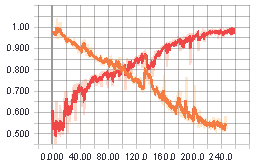
\includegraphics[scale=1.8]{Figs/graph-training-cost.pdf}
      }
      \caption{Training accuracy (red) and cost (orange) of RNN with LSTM modules.}
      \label{graph:training-lstm}
   \end{figure}




LSTM\index{Long Short-Term Memory}, using Word2Vec\index{Word2Vec}, trained on the corpus, and using the hyperparameters described above overall performed strongly when given 100 lexemes of input, coupled with a dimensionality of 100 channels. The following results describe the use of the testing datasets outlined in Section \ref{testing-methodologies}. 

The receiver operating characteristic (ROC) curve and the area under curve (AUC) were used to evaluate the effectiveness of the classifier. The ROC curve shows the trade-off between the true positive rate (TPR) and the false positive rate (FPR), and in particular is robust in the context of class imbalance \cite{japkowicz2011evaluating}. If the ROC curve is closer to the top left corner of the graph, the model is better. The AUC is the area under the curve generated. When the area is closer to 1, the model is better. AUC can be calculated as




\begin{equation}
AUC(f) = \frac{\sum_{i = 1}^{|T_{p}|}(R_i - i)}{|T_p||T_n|}
\end{equation}

Where $T_p \subset T \: and \: T_n \subset T$ are, respectively, the subsets of positive and negative examples in test set T, and $R_i$ is the rank of the \textit{i}th example in $T_p$ given by classifier \textit{f} \cite{japkowicz2011evaluating}.

    \begin{figure}[thpb]
      \centering
      \framebox{\parbox{3in}{
}
      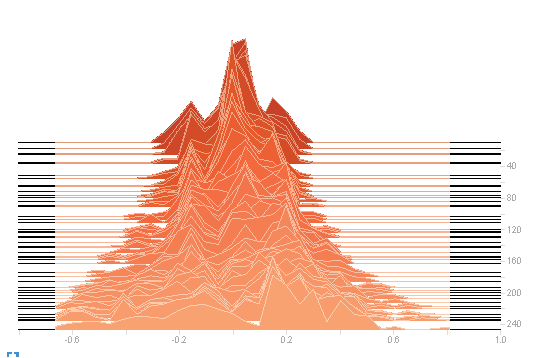
\includegraphics[scale=1.0]{Figs/histogram-tb.pdf}
      }
      \caption{Histogram displaying binned weights of LSTM model, with y-axis relating to step number.}
      \label{fig:histogram-lstm}
   \end{figure}


The hyperparamers of the networks were as defined in Table \ref{table:gating-hyperparameters}. Unless otherwise stated, the models described were tested on the Word2Vec set of word embeddings trained on the preprocessed corpus. 
 
    \begin{figure}[thpb]


      \centering
      \framebox{\parbox{3in}{
}
      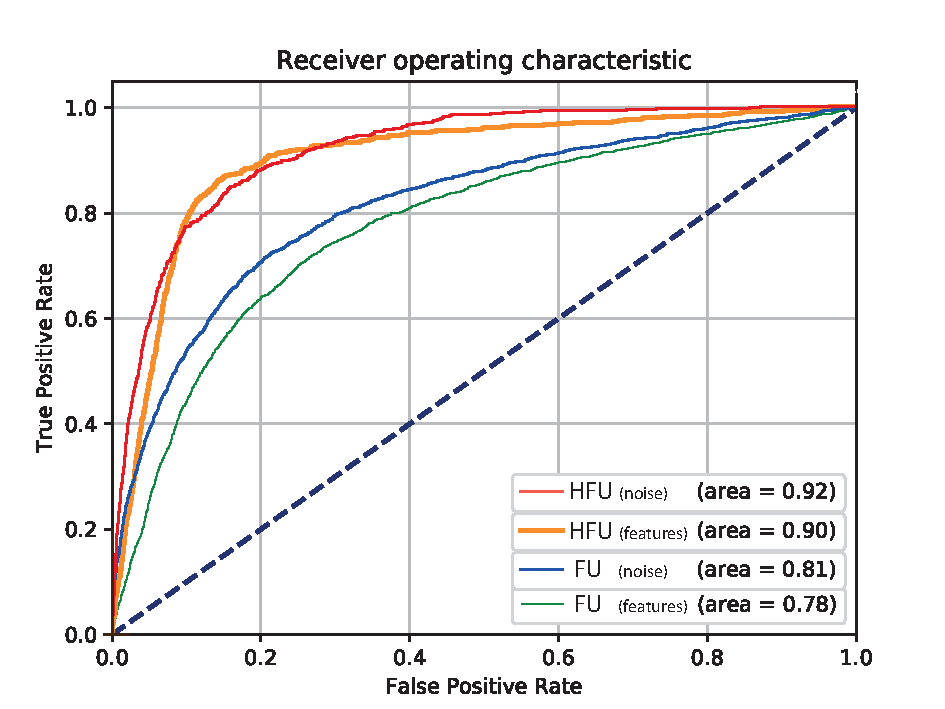
\includegraphics[scale=0.7]{Figs/graph-roc2.pdf}
      }
      \caption{ROC curve over both high frequent user cases and frequent user cases using LSTM.}
      \label{graph:roc-LSTM-noise_vs_features}
   \end{figure}



\begin{comment}
\begin{table*}[h]
   \ra{1.3}
      \centering
      \caption{Architecture and input comparison}
      \label{table:lstm-gru}
      \resizebox{\columnwidth}{!}{%

\begin{tabular}{|lll|ll|ll|ll|ll|}
\hline
   &        &      & \multicolumn{4}{c|}{LSTM}                                                                 & \multicolumn{4}{c|}{GRU\index{Gated Recurrent Units}}                                               \\\cline{4-11}
   &        &     & \multicolumn{2}{c|}{Features}                         & \multicolumn{2}{c|}{Noise}        & \multicolumn{2}{c|}{Features}      & \multicolumn{2}{c|}{Noise}         \\
T  & Length & C   & PPV                                 & NPV             & PPV             & NPV             & PPV             & NPV              & PPV             & NPV             \\ \hline
24 & 100    & 100 & \multicolumn{1}{r}{0.71$\pm 0.006$} & 0.76$\pm 0.005$ & 0.75$\pm 0.033$ & 0.75$\pm 0.047$ & 0.69$\pm 0.067$ & 0.76$\pm 0.01$   & 0.74$\pm 0.035$ & 0.74$\pm 0.035$ \\
24 & 100    & 200 & \multicolumn{1}{r}{0.73$\pm 0.021$} & 0.75$\pm 0.003$ & 0.72$\pm 0.047$ & 0.76$\pm 0.013$ & 0.74$\pm 0.009$ & 0.75$\pm 0.015$  & 0.72$\pm 0.011$ & 0.73$\pm 0.022$ \\
24 & 200    & 100 & 0.71$\pm 0.018$                     & 0.72$\pm 0.012$ & 0.54$\pm 0.21$  & 0.89$\pm 0.081$ & 0.7$\pm 0.014$  & 0.74 $\pm 0.008$ & 0.75$\pm 0.015$ & 0.74$\pm 0.01$  \\
24 & 200    & 200 & \multicolumn{1}{r}{0.78$\pm 0.098$} & 0.63$\pm 0.21$  & 0.38$\pm 0.33$  & 0.91$\pm 0.042$ & 0.78$\pm 0.083$ & 0.63$\pm 0.21$   & 0.67$\pm 0.16$  & 0.82$\pm 0.007$ \\
50 & 100    & 100 & \multicolumn{1}{r}{0.88$\pm 0.009$} & 0.78$\pm 0.008$ & 0.86$\pm 0.012$ & 0.88$\pm 0.014$ & 0.89$\pm 0.015$ & 0.8$\pm 0.013$   & 0.86$\pm 0.023$ & 0.83$\pm 0.027$ \\
50 & 100    & 200 & 0.85$\pm 0.017$                     & 0.83$\pm 0.026$ & 0.88$\pm 0.019$ & 0.84$\pm 0.025$ & 0.78$\pm 0.018$ & 0.89$\pm 0.011$  & 0.81$\pm 0.044$ & 0.86$\pm 0.041$ \\
50 & 200    & 100 & 0.80$\pm 0.083$                      & 0.69$\pm 0.23$  & 0.79$\pm 0.015$ & 0.71$\pm 0.17$  & 0.80$\pm 0.019$ & 0.65$\pm 0.26$   & 0.8 $\pm 0.32$  & 0.83$\pm 0.063$ \\
50 & 200    & 200 & 0.89$\pm 0.048$                     & 0.75$\pm 0.165$ & 0.82$\pm 0.14$  & 0.72$\pm 0.21$  & 0.83$\pm 0.22$  & 0.77$\pm 0.08$   & 0.78$\pm 0.26$  & 0.62$\pm 0.052$ \\
\hline
\end{tabular}%
}
\end{table*}
\end{comment}

\begin{table}
  \setlength{\tabcolsep}{8pt}
\centering
\caption{Architecture and input comparison: LSTM.}
\label{table-lstm}
\begin{tabular}{|lll|ll|ll|} 
\hline
   &        &     & \multicolumn{4}{c|}{LSTM}                                                                      \\ 
\cline{4-7}
   &        &     & \multicolumn{2}{c|}{Features}                           & \multicolumn{2}{c|}{Noise}           \\
T  & Length & C   & PPV                                  & NPV              & PPV              & NPV               \\ 
\hline
24 & 100    & 100 & \multicolumn{1}{r}{0.71$\pm 0.006$ } & 0.76$\pm 0.005$  & 0.75$\pm 0.033$  & 0.75$\pm 0.047$   \\
24 & 100    & 200 & \multicolumn{1}{r}{0.73$\pm 0.021$ } & 0.75$\pm 0.003$  & 0.72$\pm 0.047$  & 0.76$\pm 0.013$   \\
24 & 200    & 100 & 0.71$\pm 0.018$                      & 0.72$\pm 0.012$  & 0.54$\pm 0.21$   & 0.89$\pm 0.081$   \\
24 & 200    & 200 & \multicolumn{1}{r}{0.78$\pm 0.098$ } & 0.63$\pm 0.21$   & 0.38$\pm 0.33$   & 0.91$\pm 0.042$   \\
50 & 100    & 100 & \multicolumn{1}{r}{0.88$\pm 0.009$ } & 0.78$\pm 0.008$  & 0.86$\pm 0.012$  & 0.88$\pm 0.014$   \\
50 & 100    & 200 & 0.85$\pm 0.017$                      & 0.83$\pm 0.026$  & 0.88$\pm 0.019$  & 0.84$\pm 0.025$   \\
50 & 200    & 100 & 0.80$\pm 0.083$                      & 0.69$\pm 0.23$   & 0.79$\pm 0.015$  & 0.71$\pm 0.17$    \\
50 & 200    & 200 & 0.89$\pm 0.048$                      & 0.75$\pm 0.165$  & 0.82$\pm 0.14$   & 0.72$\pm 0.21$    \\
\hline
\end{tabular}
\end{table}


\begin{table}
  \setlength{\tabcolsep}{8pt}
\centering
\caption{Architecture and input comparison: GRU\index{Gated Recurrent Units}.}
\label{table-gru}
\begin{tabular}{|lll|ll|ll|} 
\hline
   &        &     & \multicolumn{4}{c|}{GRU}                                                    \\ 
\cline{4-7}
   &        &     & \multicolumn{2}{c|}{Features}        & \multicolumn{2}{c|}{Noise}           \\
T  & Length & C   & PPV              & NPV               & PPV              & NPV               \\ 
\hline
24 & 100    & 100 & 0.69$\pm 0.067$  & 0.76$\pm 0.01$    & 0.74$\pm 0.035$  & 0.74$\pm 0.035$   \\
24 & 100    & 200 & 0.74$\pm 0.009$  & 0.75$\pm 0.015$   & 0.72$\pm 0.011$  & 0.73$\pm 0.022$   \\
24 & 200    & 100 & 0.7$\pm 0.014$   & 0.74 $\pm 0.008$  & 0.75$\pm 0.015$  & 0.74$\pm 0.01$    \\
24 & 200    & 200 & 0.78$\pm 0.083$  & 0.63$\pm 0.21$    & 0.67$\pm 0.16$   & 0.82$\pm 0.007$   \\
50 & 100    & 100 & 0.89$\pm 0.015$  & 0.8$\pm 0.013$    & 0.86$\pm 0.023$  & 0.83$\pm 0.027$   \\
50 & 100    & 200 & 0.78$\pm 0.018$  & 0.89$\pm 0.011$   & 0.81$\pm 0.044$  & 0.86$\pm 0.041$   \\
50 & 200    & 100 & 0.80$\pm 0.019$  & 0.65$\pm 0.26$    & 0.8 $\pm 0.32$   & 0.83$\pm 0.063$   \\
50 & 200    & 200 & 0.83$\pm 0.22$   & 0.77$\pm 0.08$    & 0.78$\pm 0.26$   & 0.62$\pm 0.052$   \\
\hline
\end{tabular}
\end{table}



It was interesting that the inclusion of features provided no notable improvement in performance by either of the recurrent neural network architectures. In counterpoint, the inclusion of noise had the effect of often reducing the propensity of the classifiers to overfit (which remained an issue, even with dropout). 

The LSTM model was quite closely matched with the performance exhibited by that of the GRU\index{Gated Recurrent Units} model, as can be seen in Table \ref{table-lstm} \hl{and Table} \ref{table-gru} respectively. \hl{It was considered possible that } increasing the length of input or number of channels did not necessarily have any beneficial effect. Even where a higher percentage of true classifications were achieved in one field, there would be a corresponding decrease in true predictions in another. In particular, doubling both input length and channel size tended towards far more unstable models. 




\begin{table}[ht]
\setlength{\tabcolsep}{8pt}
   \ra{1.2}
\centering
\caption{Performance relative to age of frequent user cases.}
\label{table:age-performance}

\begin{tabular}{@{}c|ccc@{}}
\toprule
\textbf{age}           & \textbf{sensitivity} & \textbf{specificity} & \textbf{F1 score} \\ \midrule
\textit{\textgreater90} & 0.65                 & 0.67                 & 0.61              \\
\textit{80-90}         & 0.81                 & 0.77                 & 0.75              \\
\textit{70-80}         & 0.80                 & 0.72                 & 0.81              \\
\textit{60-70}         & 0.78                 & 0.71                 & 0.8               \\
\textit{50-60}         & 0.79                 & 0.7                  & 0.8               \\
\textit{40-50}         & 0.78                 & 0.73                 & 0.84              \\
\textit{30-40}         & 0.75                 & 0.75                 & 0.72              \\
\textit{20-30}         & 0.69                 & 0.76                 & 0.71              \\
\textit{10-20}         & 0.71                 & 0.94                 & 0.52              \\
\textit{\textless10}    & 0.65                 & 0.82                 & 0.61              \\ \midrule
\textbf{all}           & 0.75                 & 0.76                 & 0.76              \\ \bottomrule
\end{tabular}%

\end{table}

A high AUC was achieved for both high frequent users and frequent users with the LSTM model (using 100 channels and 100 input length based on W2V word embeddings trained on preprocessed corpus), visible in Figure \ref{graph:roc-LSTM-noise_vs_features}. The red and orange lines relate to performance for high frequent user cases, with noise or features, respectively. The blue and green lines relate to performance for frequent user cases, with noise or parameterised features, respectively.  High frequent users achieved an AUC of 0.9 (or 0.92 with noise added) and frequent users achieved an AUC of 0.78 (or 0.81 with noise added). 

While these were good results, the lack of impact made by parameterised data on the model's effectiveness was disappointing. Output from the model was also tested as a feature, provided alongside parameterised data, to both RF and SVM in the hope that these algorithms might be able to combine the effectiveness of the ANN's classification of FTN with the information contained within the parameterised data. However, no improvement on the accuracy obtained by the ANN was observed during this evaluation. 


Testing was conducted to ensure that there was no bias towards any particular type of patient. As can be seen in Table \ref{table:age-performance}, based upon validation data of frequent user cases (patients with more than 24 interactions with the OOHC), performance relating to patient age follows almost a standard deviation, with performance strongest at about the mean age of patients, and weakest towards either extreme (those less representative of the cohort as a whole).   

\begin{table}[ht]
\caption{Convolutional Layer Specifications.}
\setlength{\tabcolsep}{9pt}
\centering
\begin{tabular}{@{}lc@{}}
\toprule
     \textbf{Hyperparameter}               & \textbf{Value} \\ \midrule

Convolutional Filters           & 1              \\
Kernel Size      & 5              \\
Pool Size             & 3              \\
Dense Units            & 7                                               \\ \bottomrule
\end{tabular}%

\label{table:cnn-lstm-hyperparameters}
\end{table}



\subsection{Convolutional Layer}



Testing included the implementation of a convolutional layer with the network. CNN-LSTMs are a popular approach to similar domain problems, and can potentially produce improved results \cite{swapna2018automated,shahzadi2018cnn,
li2020hybrid}. A five layer CNN-LSTM was developed (a single convolutional layer on top of a four layer RNN\index{Recurrent Neural Network} featuring LSTM, similar in structure to that depicted in Figure \ref{fig:scheme-tensorboard}) to evaluate potential applicability with the thesis problem. Hyperparameter optimisation identified the specification detailed in Table \ref{table:cnn-lstm-hyperparameters} as best suited to the classifier.

\begin{table}[ht]
\setlength{\tabcolsep}{8pt}
   \ra{1.2}
\centering
\caption{LSTM based Network with Convolutional Layer.}
\label{table:cnn-lstm-results}
\begin{tabular}{@{}lll@{}}
\toprule
\textbf{}                & \textbf{t(24)} & \textbf{t(50)} \\ \midrule
\multicolumn{1}{l|}{PPV} & 0.70$\pm 0.03$         & 0.83 $\pm 0.04$         \\
\multicolumn{1}{l|}{NPV} & 0.82$\pm 0.039$         & 0.84 $\pm 0.02$         \\
\multicolumn{1}{l|}{TPR} & 0.1$\pm 0.01$         & 0.05 $\pm 0.17$         \\
 \bottomrule
\end{tabular}
\end{table}


Again using the testing datasets described in Section \ref{testing-methodologies} we can see that while this convolutional layer increased NPV, and reduced the propensity to overfit, this was achieved with a significant impact to positive case prediction, as shown in Table \ref{table:cnn-lstm-results}.  






\subsection{Overfitting\index{Overfitting}}

Although the model described above provided good results, during training it was clearly exhibiting strong overfitting\index{Overfitting} (visible in Figure \ref{graph:training-lstm} with corresponding updates of weights decreasing over time, visible in Figure \ref{fig:histogram-lstm}). Figure \ref{fig:histogram-lstm} \hl{depicts the rate at which the weights are being adjusted as training occurs, so it is demonstrating quite substantial speed as the weights become mostly adjusted by step 240.} The issue of overfitting was particularly relevant in relation to frequent (as opposed to high frequent) users. Increasing the volume of training examples did not affect this, nor did manually increasing dropout. Although adding noise to the input stream had helped reduce overfitting\index{Overfitting}, the use of weight decay\index{Weight decay} with Adam optimisation was examined as a potential means to improve these results. Weight decay was chosen in lieu of L2 Normalisation, as L2 Normalisation is not effective with adaptive gradient algorithms like Adam \cite{loshchilov2017fixing}.     

\begin{table}[ht]
\setlength{\tabcolsep}{8pt}
   \ra{1.2}
\centering
\caption{LSTM with weight decay.}
\label{table:weight-decay}
\begin{tabular}{@{}c|cccc@{}}
\toprule
    Value         & PPR               & NPR   & TPR     \\ \midrule
\textbf{0.1} & 0.74 $\pm 0.003$  & 0.78$\pm 0.02$ & 0.08$\pm 0.00$ \\
\textbf{0.2} & 0.72  $\pm 0.003$ & 0.79$\pm 0.03$ & 0.08$\pm 0.01$  \\
\textbf{0.3} & 0.73  $\pm 0.004$ & 0.79$\pm 0.04$ & 0.08$\pm 0.01$ \\
\textbf{0.4} & 0.74  $\pm 0.002$ & 0.78$\pm 0.04$ & 0.08$\pm 0.01$   \\
\textbf{0.5} & 0.74  $\pm 0.003$ & 0.81$\pm 0.04$ & 0.09$\pm 0.01$  \\ \
\textbf{0.6} & 0.00                 & 1          & 0.00         \\ \bottomrule
\end{tabular}
\end{table}


Experiments relating to weight decay were performed (visible in Table \ref{table:weight-decay}) with relation to a threshold of 24 cases using the testing dataset described in Section \ref{testing-methodologies} relating to this cohort. This shows that with input and channel length of 100, that for a small penalty to PPR, a statistically significant rise in NPR can be achieved. This was particularly evident with a weight decay of 0.5 (above which the model would tend towards being impossible to train). Although this provided an increase in performance at a threshold of 24 cases, no statistically significant changes were observed with high frequent user cases.

An ROC curve can be observed in Figure \ref{graph:roc-LSTM-weight-decay}, where the black plot represents frequent users, and the red plot, high frequent users.



    \begin{figure}[ht]
      \centering
      \framebox{\parbox{3in}{
}
      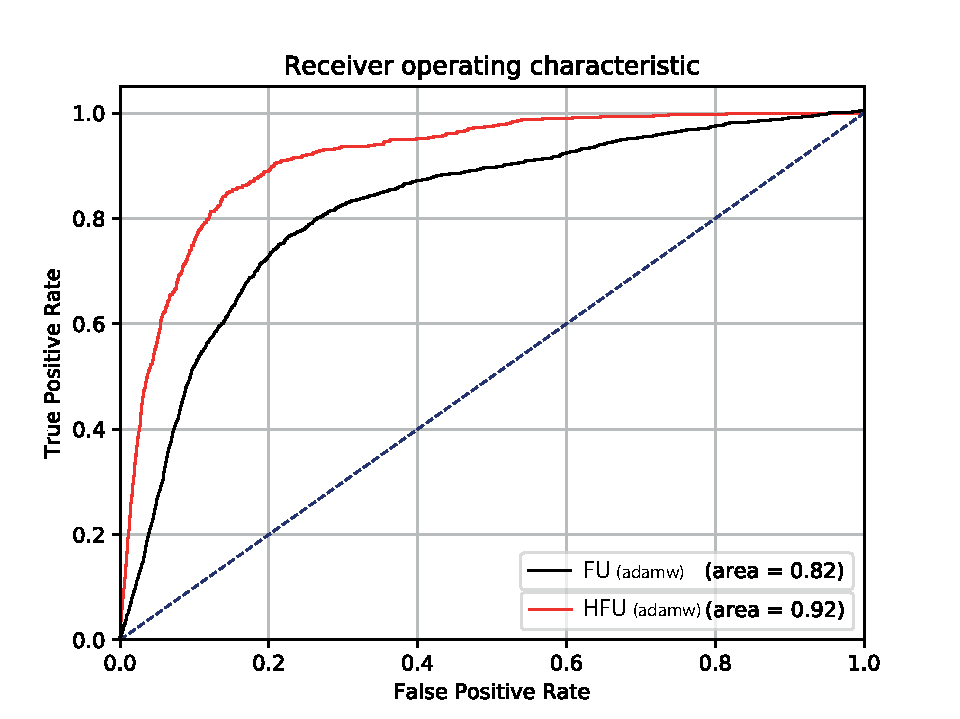
\includegraphics[scale=0.5]{Figs/graph-roc-weightdecay.pdf}
      }
      \caption{ROC curve with LSTM featuring weight decay.}
      \label{graph:roc-LSTM-weight-decay}
   \end{figure}
   
   
       \begin{figure}[ht]
      \centering
      \framebox{\parbox{3in}{
}
      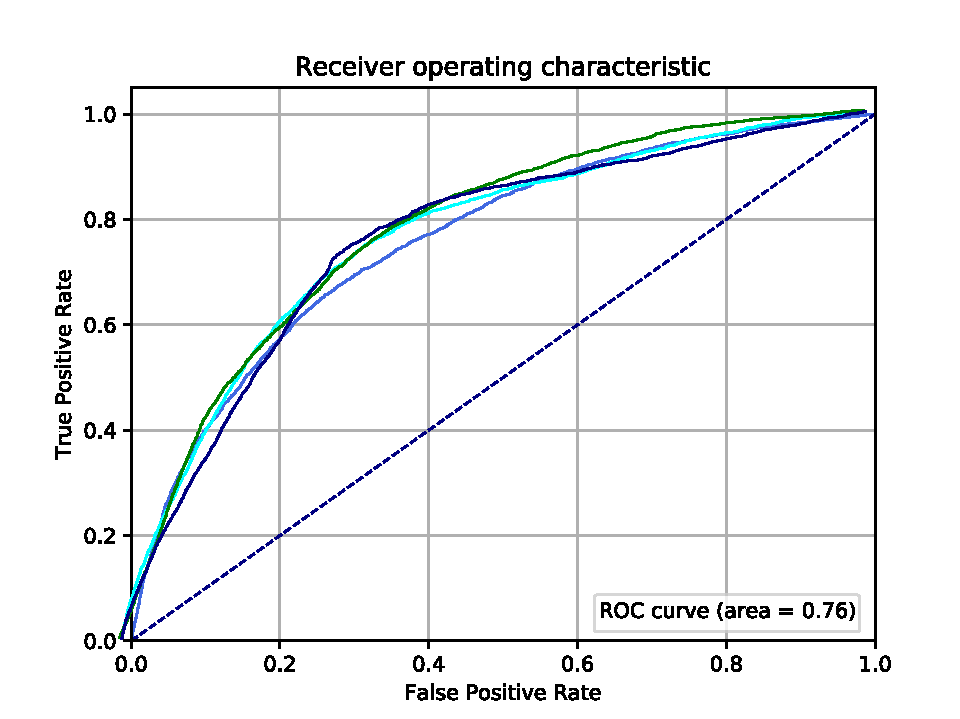
\includegraphics[scale=0.5]{Figs/graph-all-lstm-weightdecay-16threshold.pdf}
      }
      \caption{ROC curve for t(16) patients, with LSTM featuring weight decay.}
      \label{graph:roc-LSTM-16-threshold}
   \end{figure}

\begin{table}[ht]
\setlength{\tabcolsep}{8pt}
   \ra{1.2}
\centering
\caption{Testing on threshold of 16 cases.}
\label{tab:16-cases}
\begin{tabular}{@{}l|cc@{}}
\toprule
             & \textbf{Mean} & \textbf{Stdev} \\ \midrule
\textbf{PPR} & 0.71          & 0.03           \\
\textbf{NPR} & 0.70          & 0.02           \\
\textbf{TPR} & 0.10          & 0.00           \\ \bottomrule
\end{tabular}
\end{table}

\subsection{Extending threshold}
\label{extending-threshold}

The system is configurable regarding the number of calls at which a patient is considered to be a frequent caller. Although outside the scope of what this thesis considers to be a frequent user, to verify that the system's performance is not very sensitive to the threshold number, runs were conducted with patients with a threshold of 16 cases. This almost doubled the number of positive cases being considered (from 7,365 positive cases (\textit{t}(24) to 14,166). As with all other experiments described in Section \ref{RNNA}, a 50\%, 25\%, 25\% split was performed for training, validation, and testing respectively (with training and validation being a balance of positive and negative cases). Consequently 14,166 cases were used for training, 7,083  cases for validation, and 273,087 cases used for testing. The model, although performing consistently well on testing data, as seen in Figure \ref{graph:roc-LSTM-16-threshold}, nonetheless was less accurate than when a higher threshold was considered (seen in Table \ref{tab:16-cases}, over five runs). Note that Figure \ref{graph:roc-LSTM-16-threshold} displays multiple separate runs using the threshold 16 cases, with an average AUC of 0.76. This suggests that characteristics representing frequent users are less strongly exhibited in users with fewer interactions with the OOHC in question.


\subsection{Future Work}

Future work may attempt to build upon the performance of this classification program by finding alternative means to combine structured data with the successful model described in this chapter. Architectural improvements, including regularisation models, may also, hypothetically, prove beneficial. In particular the use of the attention model, though outside the scope of this research, may be used in combination with the LSTM to potentially improve results \cite{deepak2020deep,ma2018sentic,reddy2018predicting}.  





\begin{comment}


Attempts to maximise predictive accuracy and reduce overfitting\index{Overfitting} led to testing involving a combination of LSTM and CNN\index{Convolutional Neural Networks}.   on top of a CNN\index{Convolutional Neural Networks} 

Convolution layer convolve the input using pooling layers, pooling layer helps reduce the representation of input sentences, input parameters, computation in the network and control the overfitting\index{Overfitting} in the network \cite{rehman2019hybrid}. 


\begin{table}[ht]
\setlength{\tabcolsep}{9pt}
\centering
\begin{tabular}{@{}lc@{}}
\toprule
                    & \textbf{CNN-LSTM} \\ \midrule
Learning Rate       & 0.001                                                  \\
Number of Layers    & 4                                                          \\
Activation function & relu                                                      \\
Optimiser           & Adam                                                  \\
Dropout             & 0.3                                                       \\ \bottomrule
\end{tabular}%
\caption{Testing hyperparameters.}
\label{tab:my-table}
\end{table}


\begin{table}[]
\setlength{\tabcolsep}{9pt}
\centering
\caption{}
\label{table:cnn-lstm}
\begin{tabular}{@{}lc@{}}
\textbf{Hyperparameter} & \textbf{Value} \\ \midrule
Learning Rate            & 0.0093         \\
Number of Layers         & 4              \\
Convolutional Filters           & 1              \\
Kernel Size      & 5              \\
Pool Size             & 3              \\
Dense Units            & 7             
\end{tabular}
\end{table}










\end{comment}




\section{Model agnostic discussion}
\label{section:model-agnostic-explanation}





One issue with ANNs\index{Artificial Neural Networks} is their problem of interpretability. In order to improve this aspect of our program, we measured lexemes related to cases based upon whether such lexemes were within cases correctly, or incorrectly, classified by our ANN. Values from the output layer for each case classified was related to the lexemes present within these cases. These values were summed over the whole model for each lexeme, with the count being inversely proportional to how frequent each lexeme was in the corpus as a whole. More formally this can be described as
\begin{equation}
\frac{\sum \Theta_cw}{|w|} c \in C, w \in W
\end{equation}

Where $\Theta$ is the output from the neural network for a given word \textit{w}, in case \textit{c} in the corpus \textit{C}. 





Finally, in accordance with power law distribution \cite{clauset2009power},  only the lexemes which collectively represented 80\% of the entire number of words in the particular dataset were kept in order to reduce the long tail of insignificant lexemes. The resultant graph is visible in Figure \ref{fig-true-results}\footnote{Like most of the images in this thesis, this graph is vector based and should support high magnification when viewed in a digital medium.}.




True positives strongly featured the terms  `depressed', `angina', `suicidal', `gauze', `neuralgia', and `diabetic'. It is worth noting that these terms may often be subject to contextual negation in individual cases (like `patient is not suicidal'). In the case of `suicidal', approximately 25\% of the instances of this term were subject to negation. When considering the course of a patient interaction that results in these terms appearing in free text notes, it is perhaps no surprise that they bear significance, even if they are negated. While words that have strong association with psychological disorders are apparent here (including `anxiety' and `depressed') it is worth noting the terms that also seem to strongly indicate chronic disease (such as `angina', `gauze', and `diabetic'). Both these findings tie in with extant studies which have identified consistent patterns of both chronic and mental illness relating to frequent use \cite{buja2015determines}.

There were also true positive terms that were more surprising, such as `driver', `wondering', and `list'. In particular the term `said' would conventionally seem too frequent to pose much significance. However, the nature of the medical notes is important in this regard. For instance the term `said' appears a total of  2967 times in our corpus, as opposed to 2323 times for a term like `diabetic'. In other textual environments (such as social media) the relative prevalence of two terms like these would be striking. For instance, `said' is contained among the default stopwords for MyISAM search indexes \cite{mysql2019mysql}. 

True negatives for their part were strongly associated with the terms `runny', `viral', `tonsillitis', `tract', and `rash', clearing indicating infections and acute diseases. True negative cases were also strongly connected to family-orientated words, such as `mum', `dad', and `child'. It is worth pointing out that `mum' and `inflamed' also stood out among false negatives. Interestingly, `dementia' and `cancer' were two terms most strongly associated with false positives.   



Looking a bit closer at the distribution of terms relating to incorrect prediction in Figure \ref{fig-false-results}, a far tighter clumping of nodes is apparent. While this may reduce the legibility of some of the node labels, again, like with Figure \ref{fig-true-results} the most important results are those at either end of the spectrum, with the X-axis representing false positives, and the Y-axis representing false negatives. Terms that were strong predictors of both true and false positives also frequently appear in a somewhat similar position in Figure \ref{fig-false-results}. It logically follows that terms which represent strongest information gain for a classifier will also be strongly associated with false predictions when present in those contexts.

There are notable exceptions though. Although `nasal' is a term we did not see appear as strongly associated with correct answers, it is nonetheless closely related to the viral, paediatric based terms we saw in Figure \ref{fig-true-results} so strongly associated with true negatives, and its presence here among false negatives makes sense. However, there are other, more surprising terms related to false negatives. `hand', `bilateral', `talking', `severe', `town', and `nervous' are curious terms to relate to false negatives: particularly `talking' as this was very strongly associated with true positives in  Figure \ref{fig-true-results}.   


   \begin{figure*}[thpb]
   
      \centering
      \framebox{\parbox{2.5in}{
}
      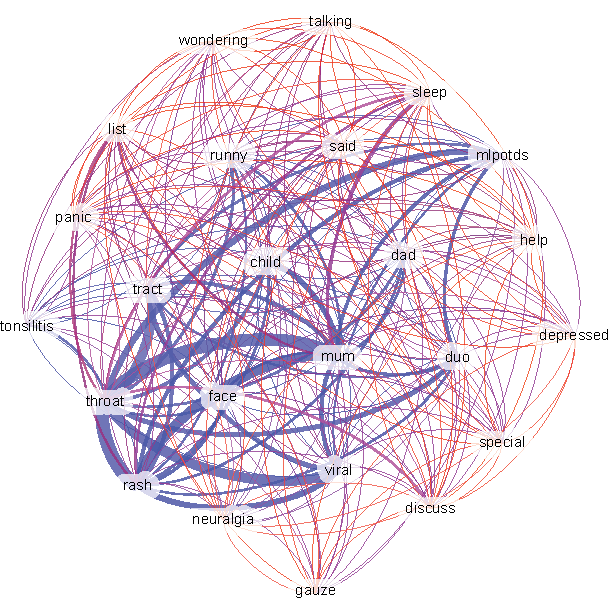
\includegraphics[page=1,width=0.96\textwidth]{network-top12-3.pdf}
      }
      \caption{Undirected graph of co-appearance of strong positive (red) and strong negative (blue) lexemes, with edge weight relative to frequency.}
      \label{fig-top-network}
   \end{figure*}


\begin{landscape}
   \begin{figure*}[thpb]
   
      \centering
      \framebox{\parbox{2.5in}{
}
      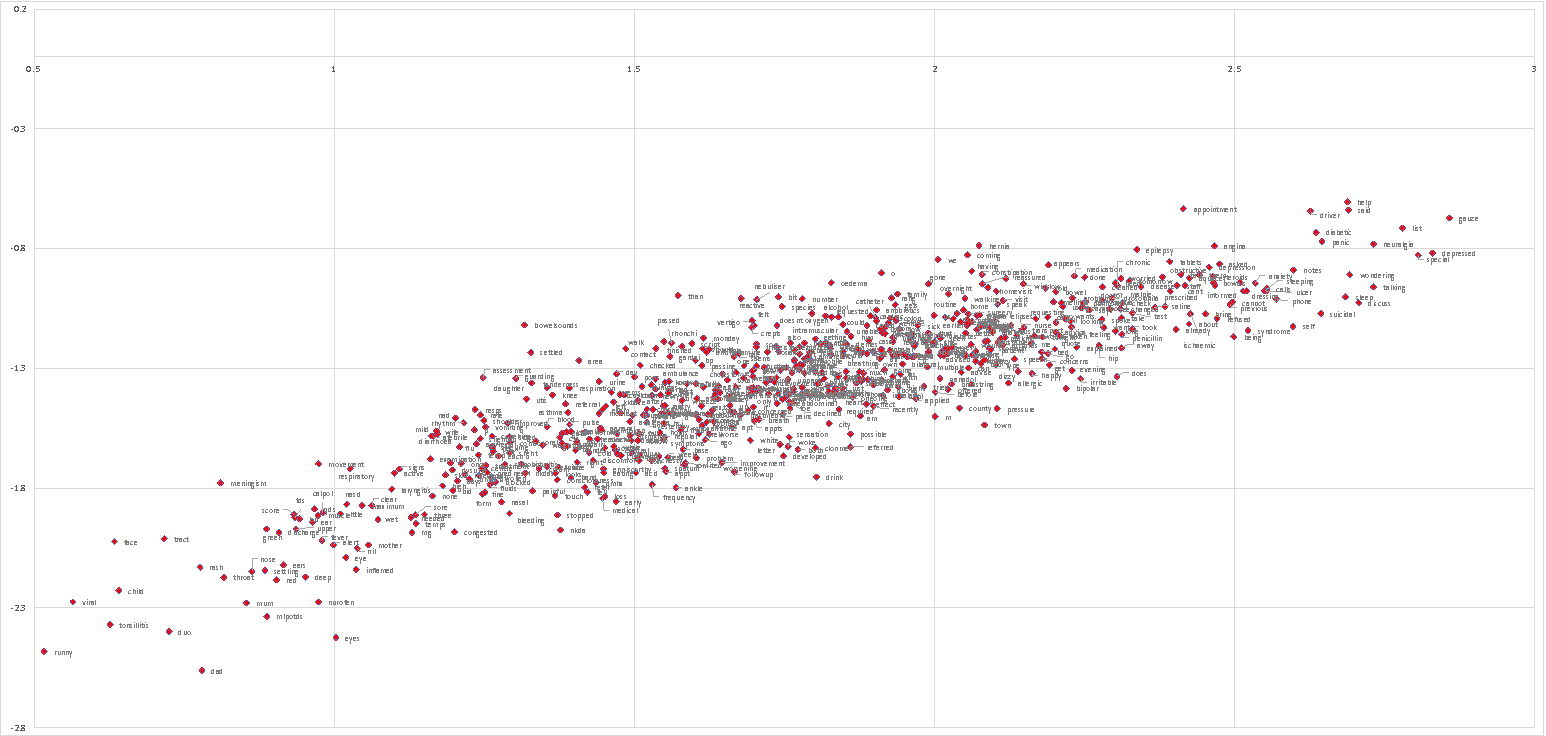
\includegraphics[page=1,width=1.8\textwidth]{24THEFULLGRAPH2.pdf}
      }
      \caption{Scatter-plot of the most significant lexemes in cases correctly classified, with the X-axis representing positive predictions, and the Y-axis representing negative predictions.}
      \label{fig-true-results}
   \end{figure*}
\end{landscape}   
   

\begin{landscape}
   \begin{figure*}[]
   
      \centering
      \framebox{\parbox{2.5in}{
}
      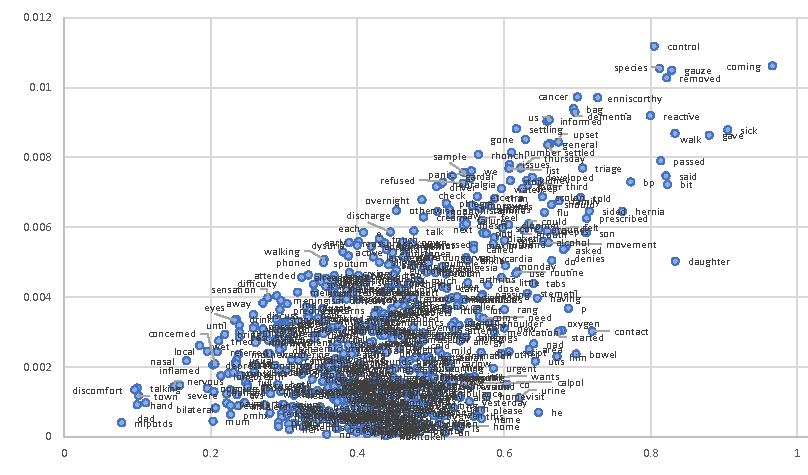
\includegraphics[page=1,width=1.8\textwidth]{24THEFULLGRAPH3s.pdf}
      }
      \caption{Scatter-plot of the most significant lexemes in cases incorrectly classified, with the X-axis representing positive predictions, and the Y-axis representing negative predictions.}
      \label{fig-false-results}
   \end{figure*}
\end{landscape} 

A contextual analysis of twelve of the top terms for true positives and true negatives can be seen in Figure \ref{fig-top-network}. This measures occurrence in sentences in all cases, irrespective of whether these cases were correctly classified. Red refers to terms which were strongly associated with true positives, blue with true negatives. Edge weight relates to frequency, while position was generated by the Yifan Hu force-directed graph drawing algorithm \cite{hu2005efficient}.    



Looking at the semantically most similar terms for these lexemes, we get a clear strong connection between some terms, like `throat' and `mum'. Both of these particular terms were strong indicators of true negatives. These two terms despite being very frequent within the corpus, are roughly equivalent to some of the far less frequent terms (like `tonsillitis') in detecting true negatives. True positive terms do not have significantly stronger connections with one another than they do to true-negative terms, based on immediate context at least.

From a word embedding perspective, some of these terms' closest neighbours can be viewed in Table \ref{table:embedding-neighbours}. Note that this is the Word2Vec\index{Word2Vec} model trained on the preprocessed version of the corpus. Though `hand' had a particularly strong association with false-negatives, its word embedding neighbours are surprisingly unremarkable (particularly given the noisy context within which the embedding model was trained).  Inspection of individual frequent user cases with respect to the word `hand' revealed that this word was used in two different contexts: to describe the location of symptoms (e.g. `left hand side' and of course, in relation to injuries to the patients' hands, for instance, as the result of a fall). Again, unusual terms are perhaps conspicuous in their absence in relation to a lexeme such as `said', which has the exact types of semantic neighbours as one would expect (that is to say, apparently generic words relating to communication). However, closer inspection of individual cases shows that the actual act of talking is of significance to some frequent users, who are a cohort more likely to suffer from loneliness and depression \cite{agarwal2019social}.


This testing shows that while lexemes indicating chronic and acute symptoms are important in identifying frequent and non-frequent patients, that both the context, and the particular sequence of words can be of particular significance. Both frequent (e.g. throat) and infrequent (e.g. tonsillitis) terms are significant when considering the role of classification with relation to frequent users.   






\begin{table}[]


      \centering
\caption{Word embedding semantic neighbours.}
\label{table:embedding-neighbours}
\resizebox{\textwidth}{!}{%
\begin{tabular}{|l|lll|}
\hline
\textbf{hand}      & `thumb':0.8670410513877869          & `wrist':0.851659893989563             & `foot':0.833329439163208           \\
\textbf{}          & `forearm':0.8140432834625244        & `elbow':0.7913630604743958            & `arm':0.7791005373001099           \\
\textbf{}          & `fingers':0.77382493019104          & `finger':0.7737174034118652           & `knuckle':0.7483718395233154       \\ \hline
\textbf{bilateral}   & `bilaterally':0.8132901787757874    & `diffuse':0.627751350402832           & `rl':0.5916634798049927            \\
\textbf{}          & `scattered':0.5810911059379578      & `global':0.5810753107070923           & `bialteral':0.5526093244552612     \\
\textbf{}          & `mild':0.5522036552429199           & `bibasal':0.5467664003372192          & `mod':0.5268542766571045           \\ \hline
\textbf{talking}   & `speaking':0.8581299781799316       & `speaks':0.7015131115913391           & `coherent':0.6972201466560364      \\
\textbf{}          & `laughing':0.6873340010643005       & `chatting':0.6761350631713867         & `conscious':0.6636359095573425     \\
\textbf{}          & `calm':0.6479660868644714           & `staring':0.6466795206069946          & `talks':0.6448451280593872         \\ \hline
\textbf{severe}    & `sever':0.769790768623352           & `intense':0.7156710624694824          & `constant':0.6517552733421326      \\
\textbf{}          & `sharp':0.6274532079696655          & `stabbing':0.6245215535163879         & `bad':0.5952492952346802           \\
\textbf{}          & `niggling':0.5927119851112366       & `colicky':0.5842158794403076          & `excruciating':0.5770964622497559  \\ \hline
\textbf{town}      & `hotel':0.5908570885658264          & `north':0.5831862688064575            & `south':0.5829253196716309         \\
\textbf{}          & `base':0.5773507356643677           & `pub':0.5677024126052856              & `hostel':0.558879017829895         \\
\textbf{}          & `park':0.5505035519599915           & `road':0.5482099056243896             & `city':0.5371564030647278          \\ \hline
\textbf{nervous}   & `system':0.6683326959609985         & `trachea':0.6188205480575562          & `TA':0.5814659595489502           \\
\textbf{}          & `neurologically':0.5766158103942871 & `gastrointestinal':0.5764801502227783 & `grossly':0.5526930689811707       \\
\textbf{}          & `peripheral':0.5519363880157471     & `central':0.5334966778755188          & `messaging':0.5289472937583923     \\ \hline
\textbf{driver}    & `receptionist':0.6956810355186462   & `dispatch':0.647824764251709          & `gardai':0.6358491778373718        \\
\textbf{}          & `reception':0.6275129914283752      & `supervisor':0.6190216541290283       & `neighbour':0.5761398673057556     \\
\textbf{}          & `carer':0.5465904474258423          & `pharmacist':0.5379290580749512       & `south':0.5368040800094604         \\ \hline
\textbf{gauze}     & `mepore':0.9428788423538208         & `mefix':0.916340172290802             & `aquacel':0.8925193548202515       \\
                   & `ribbon':0.8817423582077026         & `adaptic':0.8558177351951599          & `melolin':0.8455561995506287       \\
                   & `betadine':0.8319324254989624       & `inadine':0.8264747858047485          & `jelonet':0.8204338550567627       \\ \hline
\textbf{neuralgia} & `postherpetic':0.6631000638008118   & `trigeminal':0.6016533970832825       & `hl':0.4842143654823303            \\
                   & `consultant':0.4773425757884979     & `chiropodist':0.4571322500705719      & `trigeminus':0.45647692680358887   \\
                   & `dietician':0.45278215408325195     & `neuroglia':0.4516264796257019        & `podiatrist':0.450517475605011     \\ \hline
\textbf{viral}     & `virla':0.6982424259185791          & `virall':0.6668179035186768           & `virl':0.6483088731765747          \\
                   & `bacterial':0.6085626482963562      & `herpetic':0.5871016979217529         & `viraemia':0.5690813064575195      \\
                   & `fungal':0.5629815459251404         & `staph':0.5569247007369995            & `streptococcal':0.5457624197006226 \\ \hline
\textbf{said}      & `told':0.7658381462097168           & `stating':0.7619598507881165          & `say':0.7534968852996826           \\
                   & `saying':0.7223905324935913         & `knows':0.7186907529830933            & `says':0.7122293710708618          \\
                   & `thought':0.7096951007843018        & `mentioned':0.7039475440979004        & `advises':0.6869325637817383       \\ \hline
\end{tabular}%
}
\end{table}














\begin{comment}


   
\section{Additional Testing}

It is also the case that, notwithstanding efforts to improve the features derived from such notes, some textual notes have very little data (perhaps a couple of words at most) making the correct classification of these, in isolation, very difficult.

\begin{table}[]
\centering
\setlength{\tabcolsep}{8pt}
\begin{tabular}{cc}
\hline
\textbf{L2 Regularisation} & \textbf{Metric}      \\ \hline
1                          &                      \\
0.8                        &                      \\
0.6                        &                      \\
0.4                        &                      \\
0.2                        &                      \\
-0.2                       & \multicolumn{1}{l}{} \\
-0.4                       & \multicolumn{1}{l}{} \\
-0.6                       & \multicolumn{1}{l}{} \\
-0.8                       & \multicolumn{1}{l}{} \\
-1.0                       & \multicolumn{1}{l}{} \\ \hline
\end{tabular}%

\caption{}
\label{tab:my-table}
\end{table}


%Future work will attempt to build upon the performance of our classification program by finding alternative means to combine structured data with the successful model described in this chapter. Architectural improvements, including regularisation models, may also, hypothetically, prove beneficial.



   
   

\subsection{AdamWOptimizer}

Edit: see also this PR which just got merged into TF.
https://github.com/tensorflow/tensorflow/pull/17438

When using pure SGD (without momentum) as an optimizer, weight decay is the same thing as adding a L2-regularization term to the loss. When using any other optimizer, this is not true.


\end{comment}




\section{Summary}

This chapter detailed the development of a neural network classification system concerning frequent user cases. Several different data types were explored, along with multiple architecture options. This addressed the plurality of architecture types and data formats used in free text classification with relation to neural networks (Section \ref{section:ann-approaches}). When RNNs with word embeddings were identified as the most suitable combination for classifying frequent users, additional tests were run in relation to both these factors: subjecting both the means of preparing word embeddings, and the architecture of the RNN chosen, to a variety of different analyses. These experiments measured the impact of background corpora, of preprocessing, alternative gating techniques, the effects of weight decay, and inclusion of convolutional layers. Finally the performance of the model in relation to a different threshold of patient was examined.  Further tests observed the effects of different calibration methods employed in data preparation, as well as the potential effect of alternative gating approaches. Finally, attempts to explain the model's behaviour with relation to patients both correctly and incorrectly classified were broached, identifying several features from the FTN which pose significance in connection with the cohort being tested.   
